\documentclass[[12pt,twoside]{book}
\usepackage{_my_document_style}
\begin{document}
%
\begin{figure}[t]%[H]%[!htbp]
  \centering
  %\checkoddpage
  %\centering
    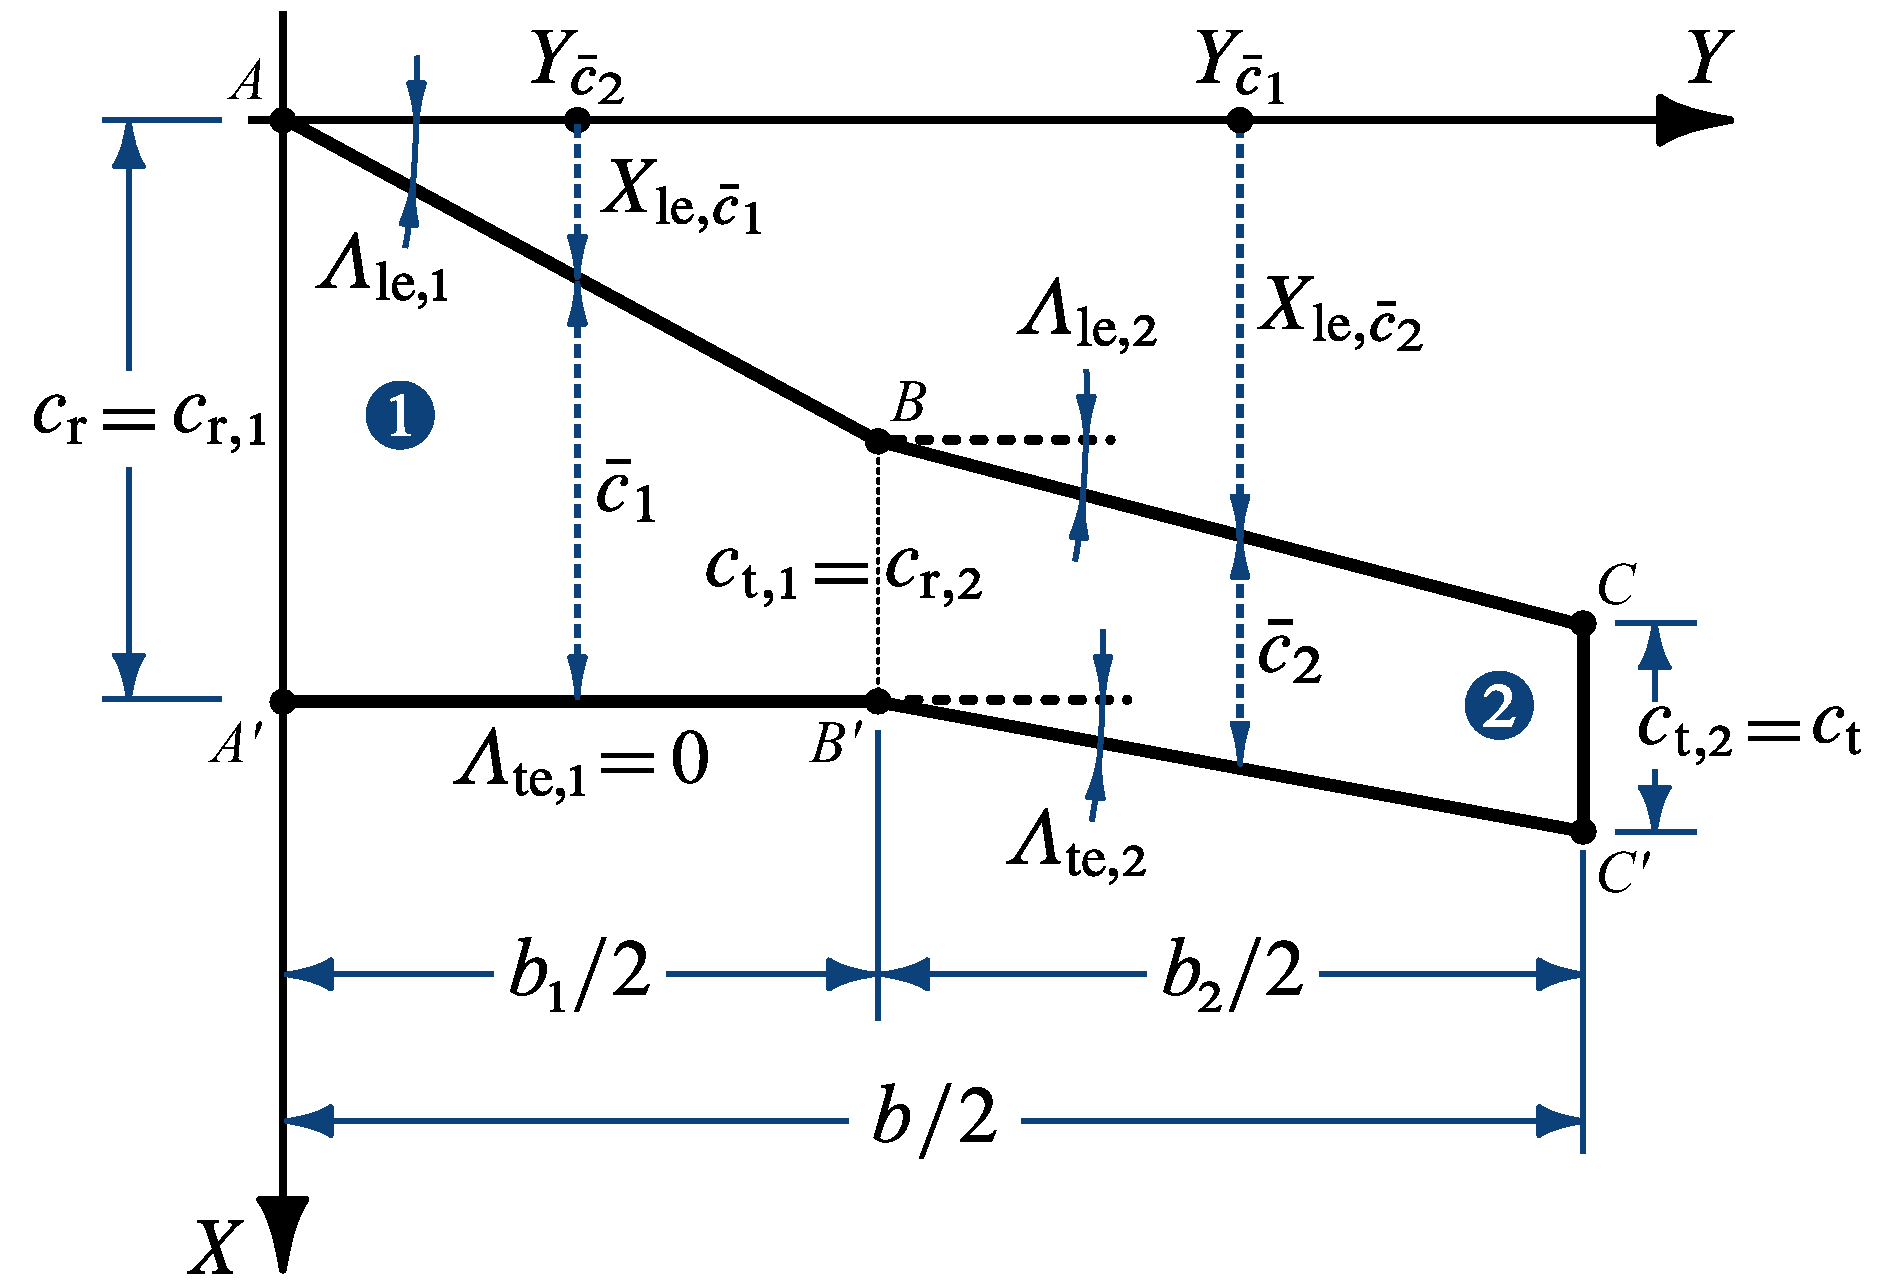
\includegraphics[width=0.78\textwidth]{Chapter_2/geometric_characteristics_of_a_cranked_wing/cranked_wing.pdf}%
  \caption{\finalhyphendemerits=1000
           Wing with not straight leading and trailing edges called cranked wing}
  \label{fig:Cranked:Wing}%
\end{figure}
%
\def\mySpanWingMT{26.800000}
\def\mySpanWingIMT{14.740000}
\def\mySpanWingIIMT{12.060000}
\def\myChordRootWingMT{5.200000}
\def\myChordRootWingIMT{5.200000}
\def\myChordRootWingIIMT{3.000000}
\def\myChordTipWingMT{2.200000}
\def\myChordTipWingIMT{3.000000}
\def\myChordTipWingIIMT{2.200000}
\def\mySweepLEWingIDEG{32.000000}
\def\mySweepLEWingIIDEG{12.000000}
\def\mySweepLEWingIRAD{0.558505}
\def\mySweepLEWingIIRAD{0.209440}
\def\myCoeffAChordWingIMT{-0.298507}
\def\myCoeffBChordWingIMT{5.200000}
\def\myCoeffAChordWingIIMT{-0.132670}
\def\myCoeffBChordWingIIMT{3.000000}
\def\myTaperRatioWingI{0.576923}
\def\myTaperRatioWingII{0.733333}
\def\myAreaWingIMTsquared{60.434000}
\def\myAreaWingIIMTsquared{31.356000}
\def\myAreaWingCrankedMTsquared{91.790000}
\def\myAspectRatioWingI{3.595122}
\def\myAspectRatioWingII{4.638462}
\def\myAspectRatioWingCranked{7.824818}
\def\myMACWingIMT{4.198374}
\def\myYMACWingIMT{3.355447}
\def\myXMACLEToApexWingIMT{2.096716}
\def\myMACWingIIMT{2.620513}
\def\myYMACWingIIMT{2.860385}
\def\myXMACLEToApexWingIIMT{0.607994}
\def\myMACWingCrankedMT{3.659367}
\def\myYYMACWingCrankedMT{5.161119}
\def\myXXMACLEToApexWingCrankedMT{3.225025}

%
\begin{myExampleX}{Geometric characteristics of a cranked wing}{\ding{46}}% \ \Keyboard\ %
\label{example:Geometric:Characteristics:Of:A:Cranked:Wing}
%
\noindent
A wing with a finite wingspan has the leading and trailing edges corresponding to two segments. In particular, the planform of the right wing is the union of two panels labeled as " panel ~ 1 " (inner panel) and " panel ~ 2 " (outer panel),
This type of planform is also called \emph{cranked wing}.
The total wingspan is $b=\SI[round-precision=1]{\mySpanWingMT}{\metre}$,
the inner panel has extension  $\frac{1}{2}b_1=\calcSI[round-precision=2,fixed-exponent=0,scientific-notation=fixed]{0.5*\mySpanWingIMT}{\metre}$,
the outer panel has extension
$\frac{1}{2}b_2=\frac{1}{2}b-\frac{1}{2}b_1
=\calcSI[round-precision=2,fixed-exponent=0,scientific-notation=fixed]{0.5*\mySpanWingIIMT}{\metre}$.
The root and tip chords are
$c_\mathrm{r}=c_{\mathrm{r},1}=\SI[round-precision=2]{\myChordRootWingMT}{\metre}$ and
$c_\mathrm{t}=c_{\mathrm{t},2}=\SI[round-precision=2]{\myChordTipWingMT}{\metre}$.
The leading edge is broken off at the point $B$
and the trailing edge is broken off at the point $B'$.
Both have coordinated
$Y_B=Y_{B'}=\frac{1}{2}b_1=\calcSI[round-precision=2,fixed-exponent=0,scientific-notation=fixed]{0.5*\mySpanWingIMT}{\metre}$.
The wing section $BB'$ has chord
$c_{\mathrm{t},1}=c_{\mathrm{r},2}=\SI[round-precision=2]{\myChordRootWingIIMT}{\metre}$.
The sweep angles of the leading edges of each panel are
$\Lambda_\mathrm{le,1}=\SI[round-precision=1]{\mySweepLEWingIDEG}{\deg}$
e $\Lambda_\mathrm{le,2}=\SI[round-precision=1]{\mySweepLEWingIIDEG}{\deg}$.

For the given \emph{cranked} wing we want to calculate the following quantities:
\noindent
\adjustbox{center=\textwidth}{%
$S$\,, $\AR$\,, $\bar{c}$\,, $X_{\mathrm{le},\bar{c}}$\,, $Y_{\bar{c}}$
}% \,, $Y_{\bar{c}}$
\medskip
The chord law of this planform is the following piecewise linear function: 
\[
c(Y)=
\begin{cases}
%\left\{
%\begin{array}{cl}
c_1(Y) = A_{c,1} \, Y + B_{c,1} & \text{for }\makebox[3em][r]{$0$}     \le Y \le \frac{1}{2}b_1
\\[4pt]
c_2(Y) = A_{c,2} \, \bigg(Y-\dfrac{b_1}{2}\bigg) + B_{c,2} & \text{for }\makebox[3em][r]{$\frac{1}{2}b_1$}< Y \le \frac{1}{2}b
\end{cases}
%\right.
\]
whose coefficients are calculated by imposing $c_1(0)=c_{\mathrm{r},1}$,
$c_1(\frac{1}{2}b_1)=c_{\mathrm{t},1}$, $c_2(\frac{1}{2}b_1)=c_{\mathrm{r},2}$, $c_2(\frac{1}{2}b)=c_{\mathrm{t},2}$.
For the given data, we have
\[
A_{c,1}
  = \frac{c_{\mathrm{t},1} - c_{\mathrm{r},1}}{b_1/2}
  = 
    2 \frac{
      \SI[round-precision=2]{\myChordTipWingIMT}{\metre} - \SI[round-precision=2]{\myChordRootWingIMT}{\metre}
    }{
      \SI[round-precision=2]{\mySpanWingIMT}{\metre}
    }
  = \mathunderline{mydarkblue}{ \SI[round-precision=3]{\myCoeffAChordWingI}{} }
\]
\[
B_{c,1}
  = c_{\mathrm{r},1}
  = \mathunderline{mydarkblue}{ \SI[round-precision=2]{\myCoeffBChordWingIMT}{\metre} }
\]
\[
A_{c,2}
  = \frac{c_{\mathrm{t},2} - c_{\mathrm{r},2}}{b_2/2}
  = 
    2 \frac{
      \SI[round-precision=2]{\myChordTipWingIIMT}{\metre} - \SI[round-precision=2]{\myChordRootWingIIMT}{\metre}
    }{
      \SI[round-precision=2]{\mySpanWingIIMT}{\metre}
    }
  = \mathunderline{mydarkblue}{ \SI[round-precision=3]{\myCoeffAChordWingII}{} }
\]
\[
B_{c,2}
  = c_{\mathrm{r},2}
  = \mathunderline{mydarkblue}{ \SI[round-precision=2]{\myCoeffBChordWingIIMT}{\metre} }
\]
So
\[
c(Y)=
\begin{cases}
%\left\{
%\begin{array}{cl}
c_1(Y) = 
  \SI[round-precision=3]{\myCoeffAChordWingI}{} \, Y 
    + \SI[round-precision=2]{\myCoeffBChordWingIIMT}{\metre} 
  & \text{per }
    \makebox[3.5em][r]{$\SI[round-precision=0]{0}{\metre}$} 
      \le Y \le 
      \calcSI[round-precision=2,fixed-exponent=0,scientific-notation=fixed]{0.5*\mySpanWingIMT}{\metre}
\\[4pt]
c_2(Y) 
  = \SI[round-precision=3]{\myCoeffAChordWingII}{} \, 
    \big(
      Y
      - \calcSI[round-precision=2,fixed-exponent=0,scientific-notation=fixed]{0.5*\mySpanWingIMT}{\metre}
    \big)
    + \SI[round-precision=2]{\myCoeffBChordWingIIMT}{\metre} 
  & \text{per }
    \makebox[3.5em][r]{%
      $\calcSI[round-precision=2,fixed-exponent=0,scientific-notation=fixed]{0.5*\mySpanWingIMT}{\metre}$
    }% end-of-makebox
      < Y 
      \le \calcSI[round-precision=2,fixed-exponent=0,scientific-notation=fixed]{0.5*\mySpanWingMT}{\metre}
%\end{array}
%\right.
\end{cases}
\]
Relative to the inner wing panel, the taper ratio is:
\[
\lambda_1
  =\frac{c_{\mathrm{t},1}}{c_{\mathrm{r},1}}
  =\frac{\SI[round-precision=2]{\myChordTipWingIMT}{\metre}}{\SI[round-precision=2]{\myChordRootWingIMT}{\metre}}
  =\mathunderline{mydarkblue}{ \SI[round-precision=2]{\myTaperRatioWingI}{} }
\]
the wing area is:
\[
\begin{split}
S_1 & {}= \frac{b_1}{2} \, c_{\mathrm{r},1} \, \big( 1 + \lambda_1 \big) \\
  & {}=
    \num{0.5} \cdot \SI[round-precision=1]{\mySpanWingIMT}{\metre}
      \cdot \SI[round-precision=2]{\myChordRootWingIMT}{\metre}
      \cdot \big( 1 + \SI[round-precision=2]{\myTaperRatioWingI}{} \big) 
    = \mathunderline{mydarkblue}{ \SI[round-precision=1]{\myAreaWingIMTsquared}{\metre^2} }
\end{split}
\]
and the corresponding wing aspect ratio is:
\[
\AR_1 
  = \frac{b_1^2}{S_1}
  = \frac{\big(\SI[round-precision=1]{\mySpanWingIMT}{\metre}\big)^2}{\SI[round-precision=1]{\myAreaWingIMTsquared}{\metre^2}}
  = \mathunderline{mydarkblue}{ \num[round-precision=2]{\myAspectRatioWingI} }
\]
%
So the mean aerodynamic chord of the inner panel is:
\[
\begin{split}
\bar{c}_1 & {}= \frac{2}{3} \, c_{\mathrm{r},1} \, \frac{1+\lambda_1 + \lambda_1^2}{1+\lambda_1} \\
  & {}=
    \num{0.667} \cdot \SI[round-precision=2]{\myChordRootWingIMT}{\metre}
      \cdot 
        \frac{
          1 + \SI[round-precision=2]{\myTaperRatioWingI}{} + \SI[round-precision=2]{\myTaperRatioWingI}{}^2
        }{
          1 + \SI[round-precision=2]{\myTaperRatioWingI}{}
        }
    = \mathunderline{mydarkblue}{ \SI[round-precision=2]{\myMACWingIMT}{\metre} }
\end{split}
\]
The longitudinal distance of the leading edge of the mean aerodynamic chord of the pannel~1 from leading edge of the root chord is
\[
\begin{split}
X_{\mathrm{le},\bar{c}_1} 
  & {}=
    \frac{b_1}{6} \, \frac{1+2\lambda_1}{1+\lambda_1} \tan\Lambda_\mathrm{le,1} \\[3pt]
  & {}=
    \frac{\SI[round-precision=1]{\mySpanWingIMT}{\metre}}{6}
      \cdot 
      \frac{
        1 + 2\cdot\SI[round-precision=2]{\myTaperRatioWingI}{}
      }{
        1 + \SI[round-precision=2]{\myTaperRatioWingI}{}
      }
      \cdot \tan \big( \SI[round-precision=3]{\mySweepLEWingIRAD}{\radian} \big)
    = \mathunderline{mydarkblue}{ \SI[round-precision=2]{\myXMACLEToApexWingIMT}{\metre} }
\end{split}
\]
The station along the opening corresponding to the chord $\bar{c}_1$ is:
\[
\begin{split}
Y_{\bar{c}_1} 
  & {}=
    \frac{b_1}{6} \, \frac{1+2\lambda_1}{1+\lambda_1} \\[3pt]
  & {}=
    \frac{\SI[round-precision=1]{\mySpanWingIMT}{\metre}}{6}
      \cdot 
      \frac{
        1 + 2\cdot\SI[round-precision=2]{\myTaperRatioWingI}{}
      }{
        1 + \SI[round-precision=2]{\myTaperRatioWingI}{}
      }
    = \mathunderline{mydarkblue}{ \SI[round-precision=2]{\myYMACWingIMT}{\metre} }
\end{split}
\]
In other words, $Y_{\bar{c}_1}$ is the distance from the center plane such that
$c_1(Y_{\bar{c}_1})=\bar{c}_1$. At this station along the wingspan corresponds a profile whose leading edge has abscissa $X_{\mathrm{le},\bar{c}_1}$.
Relative to the outer wing panel, as if it was isolated, the taper ratio is:
\[
\lambda_2
  =\frac{c_{\mathrm{t},2}}{c_{\mathrm{r},2}}
  =\frac{\SI[round-precision=2]{\myChordTipWingIIMT}{\metre}}{\SI[round-precision=2]{\myChordRootWingIIMT}{\metre}}
  =\mathunderline{mydarkblue}{ \SI[round-precision=2]{\myTaperRatioWingII}{} }
\]
the wing area is:
\[
\begin{split}
S_2 & {}= \frac{b_2}{2} \, c_{\mathrm{r},2} \, \big( 1 + \lambda_2 \big) \\
  & {}=
    \num{0.5} \cdot \SI[round-precision=1]{\mySpanWingIIMT}{\metre}
      \cdot \SI[round-precision=2]{\myChordRootWingIIMT}{\metre}
      \cdot \big( 1 + \SI[round-precision=2]{\myTaperRatioWingII}{} \big) 
    = \mathunderline{mydarkblue}{ \SI[round-precision=1]{\myAreaWingIIMTsquared}{\metre^2} }
\end{split}
\]
and the corresponding wing aspect ratio is:
\[
\AR_2 
  = \frac{b_2^2}{S_2}
  = \frac{\big(\SI[round-precision=1]{\mySpanWingIIMT}{\metre}\big)^2}{\SI[round-precision=1]{\myAreaWingIIMTsquared}{\metre^2}}
  = \mathunderline{mydarkblue}{ \num[round-precision=2]{\myAspectRatioWingII} }
\]
%
The mean aerodynamic chord of the outer panel is
\[
\begin{split}
\bar{c}_2 & {}= \frac{2}{3} \, c_{\mathrm{r},2} \, \frac{1+\lambda_2 + \lambda_2^2}{1+\lambda_2} \\
  & {}=
    \num{0.667} \cdot \SI[round-precision=2]{\myChordRootWingIIMT}{\metre}
      \cdot 
        \frac{
          1 + \SI[round-precision=2]{\myTaperRatioWingII}{} + \SI[round-precision=2]{\myTaperRatioWingII}{}^2
        }{
          1 + \SI[round-precision=2]{\myTaperRatioWingII}{}
        }
    = \mathunderline{mydarkblue}{ \SI[round-precision=2]{\myMACWingIIMT}{\metre} }
\end{split}
\]
%
The longitudinal distance of the leading edge of mean aerodynamic chord of the panel~2 from
point $B$ is:
\[
\begin{split}
X_{\mathrm{le},\bar{c}_2} - X_B
  & {}=
    \frac{b_2}{6} \, \frac{1+2\lambda_2}{1+\lambda_2} \tan\Lambda_\mathrm{le,2} \\[3pt]
  & {}=
    \frac{\SI[round-precision=1]{\mySpanWingIIMT}{\metre}}{6}
      \cdot 
      \frac{
        1 + 2\cdot\SI[round-precision=2]{\myTaperRatioWingII}{}
      }{
        1 + \SI[round-precision=2]{\myTaperRatioWingII}{}
      }
      \cdot \tan \big( \SI[round-precision=3]{\mySweepLEWingIIRAD}{\radian} \big)
    = \mathunderline{mydarkblue}{ \SI[round-precision=2]{\myXMACLEToApexWingIIMT}{\metre} }
\end{split}
\]
%
This distance is the one that would be calculated if the wing coincided with the outer panel
that is if $B$ were the leading edge of the root chord. So the abscissa $X_{\mathrm{le},\bar{c}_2}$ is:
\[
\begin{split}
X_{\mathrm{le},\bar{c}_2} & {}= X_B + \SI[round-precision=2]{\myXMACLEToApexWingIIMT}{\metre}
  = \frac{b_1}{2} \tan \Lambda_{\mathrm{le},1} + \SI[round-precision=2]{\myXMACLEToApexWingIIMT}{\metre}
\\
  & {}= \calcSI[round-precision=2,fixed-exponent=0,scientific-notation=fixed]{
          0.5 * \mySpanWingIMT
        }{\metre}
       \cdot \tan( \SI[round-precision=3]{\mySweepLEWingIRAD}{\radian} )
      + \SI[round-precision=2]{\myXMACLEToApexWingIIMT}{\metre}
    = \calcSI[round-precision=2,fixed-exponent=0,scientific-notation=fixed]{
          0.5 * \mySpanWingIMT * tan( \mySweepLEWingIRAD )
        }{\metre}
      + \SI[round-precision=2]{\myXMACLEToApexWingIIMT}{\metre}
    = \mathunderline{mydarkblue}{ 
      \calcSI[round-precision=2,fixed-exponent=0,scientific-notation=fixed]{
          0.5 * \mySpanWingIMT * tan( \mySweepLEWingIRAD )
          + \myXMACLEToApexWingIIMT
      }{\metre}
    }
\end{split}
\]
The station along the wingspan corresponding to the chord $\bar{c}_2$ is:
\[
\begin{split}
Y_{\bar{c}_2} 
  & {}=
    \frac{b_1}{2} + 
    \frac{b_2}{6} \, \frac{1+2\lambda_2}{1+\lambda_2} \\[3pt]
  & {}=
    \calcSI[round-precision=2]{0.5*\mySpanWingIMT}{\metre} +
    \frac{\SI[round-precision=1]{\mySpanWingIIMT}{\metre}}{6}
      \cdot 
      \frac{
        1 + 2\cdot\SI[round-precision=2]{\myTaperRatioWingII}{}
      }{
        1 + \SI[round-precision=2]{\myTaperRatioWingII}{}
      }
    = \mathunderline{mydarkblue}{
      \calcSI[round-precision=2]{0.5*\mySpanWingIMT}{\metre} +
      \SI[round-precision=2]{\myYMACWingIIMT}{\metre} 
    }
    = \mathunderline{mydarkblue}{
      \calcSI[round-precision=2,fixed-exponent=0,scientific-notation=fixed]{0.5*\mySpanWingIMT + \myYMACWingIIMT}{\metre}
    }
\end{split}
\]
%
This is the true distance from the symmetry plane of the wing station in the outer panel with chord equal to $\bar{c}_2$.
The assigned planform has a total surface area equal to:
\[
S = S_1 + S_2
  = \SI[round-precision=1]{\myAreaWingIMTsquared}{\metre^2}
    = \mathunderline{mydarkblue}{
      \SI[round-precision=1]{\myAreaWingCrankedMTsquared}{\metre^2}
    }
\]
and aspect ratio:
\[
\AR = \frac{b^2}{S} 
    = \frac{
        \big( \SI[round-precision=2]{\mySpanWingMT}{\meter} \big)^2
      }{
        \SI[round-precision=1]{\myAreaWingCrankedMTsquared}{\metre^2}
      }
    = \mathunderline{mydarkblue}{
      \SI[round-precision=2]{\myAspectRatioWingCranked}{}
    }
\]
From the general formula for calculating the mean aerodynamic chord written for a \emph{cranked} wing with two panels:
\[
\bar{c} 
  = \frac{1}{S} \int_0^{b/2} c^2(Y) \diff{Y} 
  = \frac{1}{S} \int_0^{b_1/2} c_1^2(Y) \diff{Y} 
    + \frac{1}{S} \int_{b_1/2}^{b/2} c_2^2(Y) \diff{Y}
\]
being the two integrals on the second side equal to $S_1 \, \bar{c}_1$ e $S_2 \, \bar{c}_2$, respectively, we have that $\bar{c}$ of the given wing is given by the following weighted average:
\[
\bar{c} = \frac{S_1 \, \bar{c}_1 + S_2 \, \bar{c}_2} {S_1 + S_2}
  =
  \frac{\SI[round-precision=1]{\myAreaWingIMTsquared}{\metre^2} \cdot \SI[round-precision=2]{\myMACWingIMT}{\metre} + \SI[round-precision=1]{\myAreaWingIIMTsquared}{\metre^2} \cdot \SI[round-precision=2]{\myMACWingIIMT}{\metre}}{\SI[round-precision=1]{\myAreaWingIMTsquared}{\metre^2} + \SI[round-precision=1]{\myAreaWingIIMTsquared}{\metre^2}}
    = \mathunderline{mydarkblue}{ \SI[round-precision=2]{\myMACWingCrankedMT}{\metre} }
\]
It is observed that $\bar{c} > c_{\mathrm{t}.1}$, being $S_1>S_2$.Therefore, the value of the station $Y_{\bar{c}}$ must be searched for among the coordinates $Y$ of the profiles mounted along the inner panel,that is, looking at the law of the chords $c_1(Y)$. So we obtain
\[
\bar{c}=A_{c,1}\,Y_{\bar{c}} + B_{c,1} \quad \Rightarrow \quad
  Y_{\bar{c}} 
    = \frac{\bar{c} - B_{c,1}}{A_{c,1}}
    = \frac{
      \SI[round-precision=2]{\myMACWingCrankedMT}{\metre} 
        - \SI[round-precision=2]{\myCoeffBChordWingIMT}{\metre}
      }{
        \SI[round-precision=3]{\myCoeffAChordWingI}{}
      }
    = \mathunderline{mydarkblue}{
      \SI[round-precision=2]{\myYYMACWingCrankedMT}{\metre}
    }
\]
Once this station has been identified, the calculated coordinate is $X$ of the leading edge
of the corresponding chord, that is $X_{\mathrm{le},\bar{c}}$.
The longitudinal distance of the leading edge of the \emph{cranked} wing mean aerodynamic chord  from leading edge of the root chord is in this case
\[
X_{\mathrm{le},\bar{c}} 
  = Y_{\bar{c}} \tan \Lambda_{\mathrm{le},1}
  = \SI[round-precision=2]{\myYYMACWingCrankedMT}{\metre}
    \cdot \tan( \SI[round-precision=3]{\mySweepLEWingIRAD}{\radian} )
  = \mathunderline{mydarkblue}{ \SI[round-precision=2]{\myXXMACLEToApexWingCrankedMT}{\metre} }
\]

\begin{figure}[t]%[H]%[!htbp]
  %\centering
  %\checkoddpage
  %\centering
    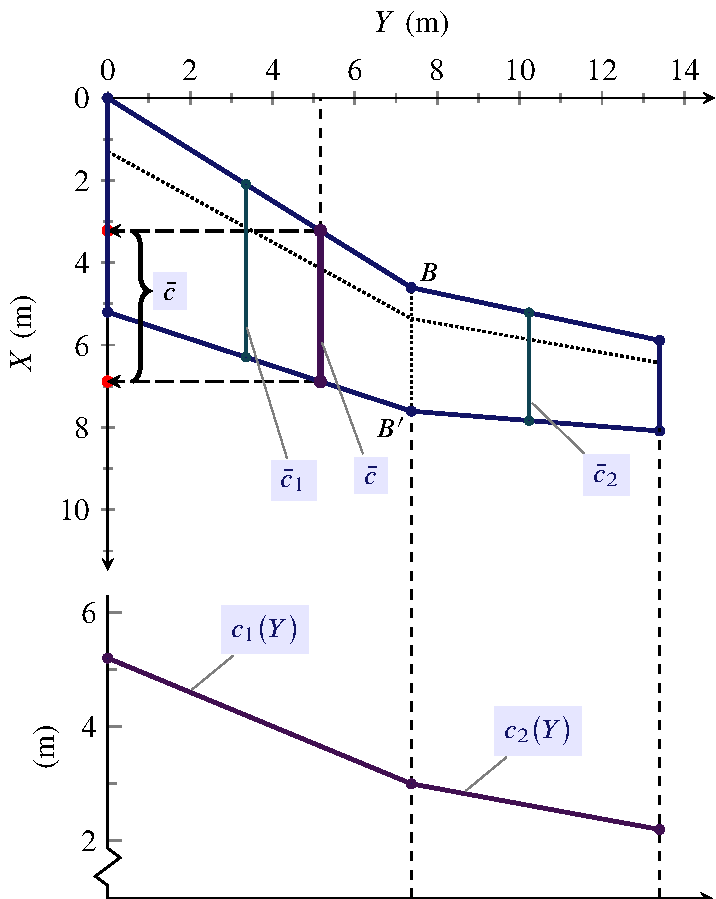
\includegraphics[width=0.78\textwidth]{Chapter_2/geometric_characteristics_of_a_cranked_wing/wing_planform_basic_2_drawing.pdf}%
  \caption{\finalhyphendemerits=1000
           Planform of the  \emph{cranked} wing assigned in the example~\ref{example:Geometric:Characteristics:Of:A:Cranked:Wing}.
           The piecewise linear chord law is also reported.
  }
  \label{fig:Cranked:Wing:Planform:Results}%
\end{figure}
\end{myExampleX}
\end{document} 
